\chapter*{Data acquisition}
ToDo:
\begin{itemize}
  \item Aus deutsch ins englische übersetzen.
  \item Beim vorletzten Punkt, die Zutaten Tools und Container besser beschreiben.
  \item Tabelle der Videos vervollständigen.
  \item Code Bild um Stir vervollständigen. 
\end{itemize}
A part of this master's thesis involves creating a knowledge base that includes certain queryable parameters, allowing the robot to perform specific actions. The initial step in building the knowledge base is to gather data. In this chapter, we elaborate on our data acquisition strategy.
\section*{Task variations}
	As our main focus is to represent the knowledge about mixing, first we had to acquire the different types and variations of mixing in order to create a complete Knowldegerepresentation. The first step in acquiring the needed data, was to acknowledge which task varations of mixing are actually important. 
  So we had to analyze the word \textit{Mixing} and its hyponyms. But first we have to ask ourselves What is Mixing?
  \subsection*{What is Mixing?}
  The definition provided by the Oxford Dictionary is as follows: To put together or combine (two or more substances or things) so that the constituents or particles of each are interspersed or diffused more or less evenly among those of the rest; to unite (one or more substances or things) in this manner with another or others; to make a mixture of, to mingle, blend.
  Ultimately, this definition conveys that mixing requires at least two elements or substances, which are then combined (evenly) with each other, resulting in a (new) substance.
  This definition is general and can be applied to various contexts. For our work, the aspect of cooking or mixing different (cooking) ingredients is important. Therefore, we consider some hyponyms of the verb "mixing" irrelevant for our cause and do not take them into account.
  An adapted definition for our work could be: Mixing is the combination of various (cooking) ingredients through different motions in a container.
  
  \subsection*{Mixing hyponyms analysis} 
	Hyponyms are subordered words of a given word, for example one hyponym of mixing could be beating. 
  To conduct this analysis, one can utilize tools from various websites, such as FrameNet and WordNet. These platforms provide users with the ability to search for specific words and obtain various associations for those words, including synonyms, acronyms, or, crucial for our case, hyponyms.	
  \subsubsection*{WikiHow extraction}
  For all those hyponyms, we delegated a WikiHow extraction search which should show us, how many times one of these words occur, in the context of cooking.
	Damit wir die Suche ausführen können definieren wir eine neue Klasse "MixingVerb", welche das Verb Mix, sowie die von uns gefundenen hyponyme und Synonyme enthält.
  \begin{figure}[H]
    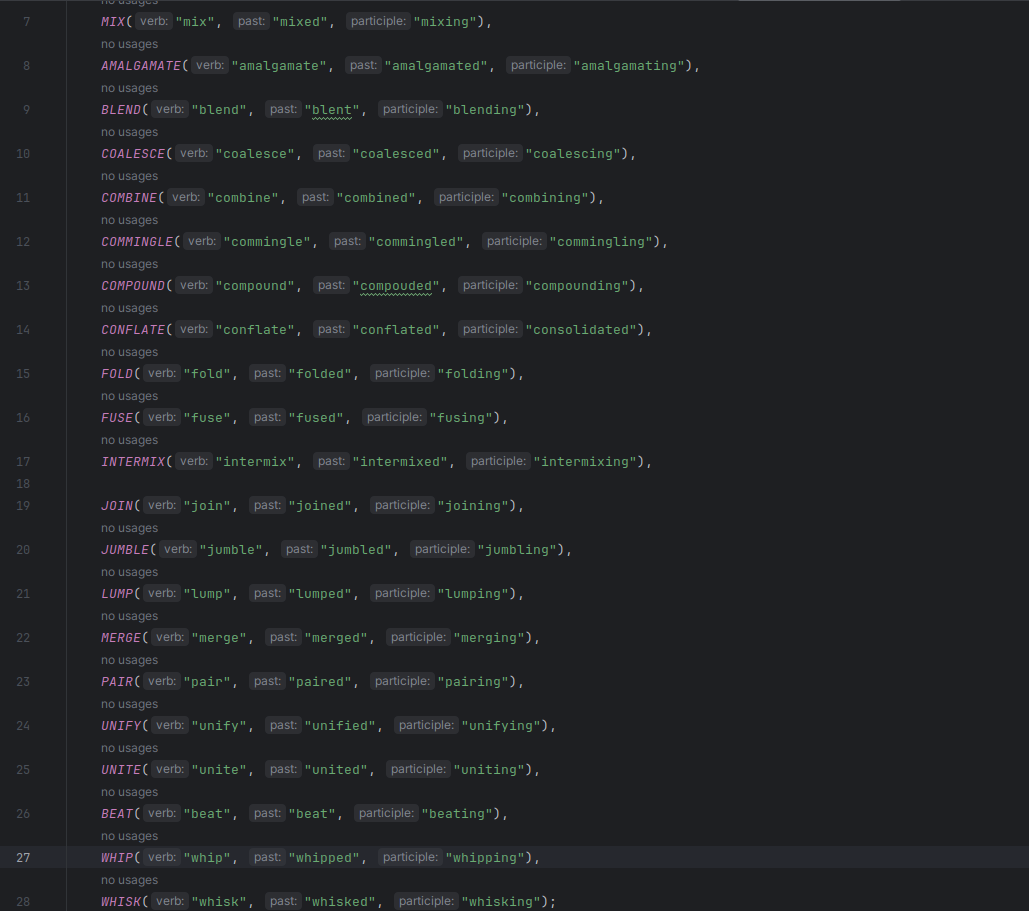
\includegraphics[scale=0.3]{Graphics/MixingVerbClass.png}
    \end{figure}
    IN DEM BILD FEHLT STIRRING
  Da wir nun die gewünschten Verben, wonach wir letzendlich suchen möchten definiert haben, passen wir einige Suchparameter für die Suche an.
  Die wichtigen Parameter sind das Filtern der Kategorien, in unserem Fall möchten wir uns auf das Mixen in dem Kochbereich fokussieren, deshalb filtern wir alle Artikel, welche nicht in dem Bereich Food and Entertaining existieren, aus.
  \subsubsection*{Hyponyms occurance}
  Für jedes definierte Verb, wird eine Suche gestartet, wie oft dieses Verb in den WikiHow Artikeln vorkommt, dadurch wollen wir in Erfahrung bringen, welche Verben letzendlich für unsere Implentierung relevant sind und welche wir ausschließen können, da sie selten vorkommen im alltäglichen Gebrauch.
  In the table below the results can be seen.
    \begin{table}[H]
        \centering
        \begin{tabular}{|c|c|}
          \hline
          \textbf{Hyponym} & \textbf{Occurance}  \\
          \hline
          Mix & 5300 \\
          \hline
          Amalgamate & 0 \\
          \hline
          Beat & 956 \\
          \hline
          Blend & 1041 \\
          \hline
          Coalesce & 1 \\
          \hline
          Combining & 3591  \\
          \hline
          Coommingle & 0 \\
          \hline
          Compound & 0 \\
          \hline
          Conflate & 0 \\
          \hline
          Folding & 821 \\
          \hline
          Fuse & 17 \\
          \hline
          Intermix & 0 \\
          \hline
          Join & 53 \\
          \hline
          Jumble & 0 \\
          \hline
          Lump & 7 \\
          \hline
          Merge & 6 \\
          \hline
          Pair & 352 \\
          \hline
          Stir & 6027 \\
          \hline
          Unify & 2 \\
          \hline
          Unite & 2 \\
          \hline
          Whip & 863 \\
          \hline
          Whisk & 2267 \\
          \hline
          
    
        \end{tabular}
        \caption{Mix synoyms/hyponyms occurance}
        \label{tab:example}
      \end{table}
      
  \subsubsection*{Further examination and conclusion}
  Diese Suche soll uns letzendlich Auskunft darüber geben, welche Verben wir in der Wissensbasis repräsentieren wollen, daher entscheiden wir uns für gewisse Verben unter 2 Bedingungen, Häufigkeit und Ausführbarkeit. Die erste Bedingung ist leicht zu verstehen, Verben die gar nicht oder so gut wie gar nicht vorkommen, werden nicht in Betracht gezogen. Die zweite Bedingung bezieht sich auf die Ausführbarkeit des Verbs im Kontext von Roboternbewegungen. Außerdem werden einige Verben mit relativ hoher Häufigkeit auch etwas genauer untersucht, da im Englischen der past tense auch als adjektiv benutzt wird unter gewissen Umständen.
  Unter Berücksichtigung der ersten Bedingung werden folgende Verben nicht in Betracht gezogen: Amalgamate, Coalesce, Comingle, Compound, Conflate, Fuse, Intermix, Join, Jumble, Lump, Merge, Unify und Unite.
  Die zweite Bedingung schließt ein weiteres Verb aus: Blend. Blend wird meistens nur im Kontext mit einer Blendmaschine benutzt, welches vom Roboter nicht gehandhabt wird. Ohne diese Maschine kann die Blend-Ausführung nicht richtig durchgeführt werden und somit ist für uns dieses Verb ausgeschlossen.
  Unter genauer Betrachtung werden wir auch das Verb Whip nicht in Betracht ziehen, da dieses meist als adjektiv von Zutaten genutzt wird, wie zum Beispiel whipped Cream. Dies stellt heraus, dass nur das Verb Whip eine relativ gerine Häufigkeit hat. Das selbe gilt für pair, wo das past tense dazu genutzt wird eine Verbindung von verschiedenen Zutaten zu beschreiben, Wine paired with cheese.

  Somit sind die von uns in Betracht gezogenen Verben: Mix, Combine, Beat, Fold, Stir und Whisk.
  

  \section*{Task analysis and defintion}
  Da wir nun die Tasks ausgewählt haben, müssen diese Tasks anaylsiert werden und geschaut werden in welchem Kontext sie letzendlich genutzt werden. Unser Ziel ist es, dass der Roboter diese Tasks so ausführen kann, wie ein Mensch es tun würde. Um dies zu bewerkstelligen müssen wir im nächsten Schritt diese Tasks näher untersuchen. Dazu empfiehlt es sich Videos auf WikiHow oder andere Quellen zu analysieren, wo diese Tasks als Aufgabe vorkommen. Die Analyse besteht daraus zu gucken mit welchen Bewegungen die Tasks in Verbindung gebracht werden. Diese Analysen stellen wir tabellarisch im Folgenden dar. Untersucht wird die Task an sich, die jeweiligen Zutaten die verarbeitet werden, die Tools die dafür genutzt werden, sowie der Behälter worin die Task ausgeführt wird. 
  \begin{table}[H]
    \centering
    \begin{tabular}{|c|c|c|p{4,5cm}|p{4,5cm}|}
        \hline
        \textbf{Task} & \textbf{Tool} & \textbf{Container} & \textbf{Ingredients} & \textbf{Description} \\
        \hline
        Beating & Whisk & Bowl & Egg yolk (Wet ingredient) & circular, swirling wildly around the bowl \\
        \hline
        Stirring & Whisk & Bowl & Beaten Egg Yolk (Wet), Parmesan(Powder) and Pepper (Powder) & Circular, from the inside to the outside. \\
        \hline
        Stirring & Tongs & Pan & Wet Mixture, Pasta (Solid) and Bacon (Solid) & Diving motions, circular but also straight lines. \\
        \hline
        Whisk & Fork & Bowl & Eggs (Wet) & Circular but also straight, wildly motion. \\
        \hline
        Mixing & Spatula & Pan & Eggs, melted butter (Wet) & Circular, from the inside to the outside, also diving. \\
        \hline
        Folding & Spatula & Pan & cooked eggs in melted butter (Wet) & Gently motion from the outisde to the inside straight, then moving about 90 degree before going to the inside again. \\
        \hline
        Mixing & Spoon & Cup & Dry yeast(Powder), Water (Liquid) & Circular \\
        \hline
        Mixing & Spoon & Bowl & Dry yeast, Water, Flour (Powder), Salt(Powder) & Whirlstorm-like motion. \\
        \hline 
    \end{tabular}
    \caption{Video analysis}
    \label{tab:example}
  \end{table}
NOCH UNVOLLSTÄDNIG

Nach einer genauen Analyse der Videos und der in den Videos bereitgestellten Informationen, schlussfolgern wir, dass die ausgeführte Bewegung nicht nur im Zusammenhang mit dem Task steht, sondern auch mit den genutzten Zutaten. Einige Tasks sind allerdings determinierend, im Sinne dass sie schon ohne unbedingt auf die Zutaten zu achten, die Bewegung zwingend ausgeführt wird.
Im Folgenden wollen wir extrahierten Informationen aus den Videos strukturieren und unsere Ergebnisse vorstellen
\subsection*{Video analysis conclusion and results}

Basierend auf den extrahierten Informaitonen schlussfolgern wir dass für unsere Ziele folgende Aspekte, neben der Task, wichtig sind und weiter betrachtet werden:
\begin{itemize}
  \item Ingredients: Die Zutaten spielen bei der Bewegungsentscheidung im Zusammenhang mit den Tasks eine wichtige Rolle und werden genauer definiert.
  \item Tools: Die Tools die genutzt werden sind bei der Bewegungsentscheidung nicht unbedingt ausschlaggebend, diese sind jedoch wichtig für die Paramter des Roboters????
  \item Container: Das selbe wie oben.
  \item Motions: Die Motions stellen letzendlich die Bewegung des Roboters für unsere Implentierung dar. Diese Bewegungen werden aus den Videos extrahiert und auf Roboternbewegungen abstimmend definiert.
\end{itemize}

\subsubsection*{Ingredients}
Durch die Videoanalyse gelangen wir zu der Schlussfolgerung, dass die Zutaten wichtig sind gegeben dessen Art. Wir unterscheiden bei den Zutaten zwischen 4 Arten:
Wet, Solid, Dry/Powder und Liquid. Somit ist letzendlich nicht die Zutat an sich wichtig sondern dessen Art.
Hier eventuell die WhatToMake Ontology nehmen und subClassOf machen?

\subsubsection*{Tools and Container}
Das kommt von Soma, muss man schauen wie man das beschreiben möchten

\subsubsection*{Motions}
	From this videos we extracted informations about the executed motions. The following motions can be defined:
	\begin{itemize}
		\item \textbf{Circular}: Moving the tool in a defined circular movement in the container, not changing the radius during execution
		\item \textbf{Whirlstorm}: Moving from the inside to the outside of the container with the tool, by circulating in an incremented radius.
		\item \textbf{Folding}: Gently motion, where you start from the outside, moving one straight line to the inner side, then picking the tool up and going to the initial state before moving the tool for about 90 degrees, then going back in a straight line to the inner side of the container again.
		\item \textbf{VerticalCircular}: Imagine a line which can be seen as the diameter of the container, from this line one can define certain regions on which you move the tool circular from side to side. This motion is used by the beating task.
		\item \textbf{CircularDivingToInner}: Starting from the outerside, moving the tool in the container arround its edge for about 270 degrees, before diving to the middle of the container. This motion is used by Tasks where is required to turn the Ingredients over.
	\end{itemize}

\section*{Data Acquision Conclusion}

Bei der Datenacquise fokussierten wir uns darauf eine Grundlage der benötigen Daten und Informationen zu erschaffen, welche für einen Roboter benötigt werden verschiedene Mixing Tasks auszuführen.
Nach der Feststellung der Tasks, konnten wir Videos analysieren um die Bewegungen zu untersuchen die in Zusammenhang mit den jeweiligen Tasks stehen. Dabei sind wir zu dem Entschluss gekommen, dass nicht nur die Task ausschlaggebend für die Bewegung sei, sondern auch die Zutatenauswahl.
Die Zutaten werden in 4 verschiedenen Kategorien unterteilt und wir konnten 5 Motions definieren, welche vom Roboter so ausgeführt werden sollen, wie es im Alltag gebräuchlich ist.
Im nächsten Kapitel wollen wir vorstellen, wie wir dieses Wissen nun repräsentieren und ein System erstellen, wodurch der Roboter in der Lage ist zu Wissen welche Bewegung es ausführen soll basierend auf einer gegebenen Task und Zutaten.
\newpage
\section*{Decision Trees}
In this section we want to illustrate the decision tree for the ellaborated tasks, starting with the Mixing task.
This trees should decide which motion is used for given Task and Ingredients combinations, as well as which Tool and Container would be preffered.
For example if we regard the combination of: \newline Task: Mixing + Ingredients: Wet and Liquid -> WhirlstormMotion. The preffered Container would be the bowl, and the preffered tools would be the spoon and whisk.
Some Tasks do not contain every possible Ingredients combinations, so the Decision Trees might be uncompleted. We also regard the Combining task eqully to the Mixing task.

\subsection*{Mixing}
\begin{figure}[H]
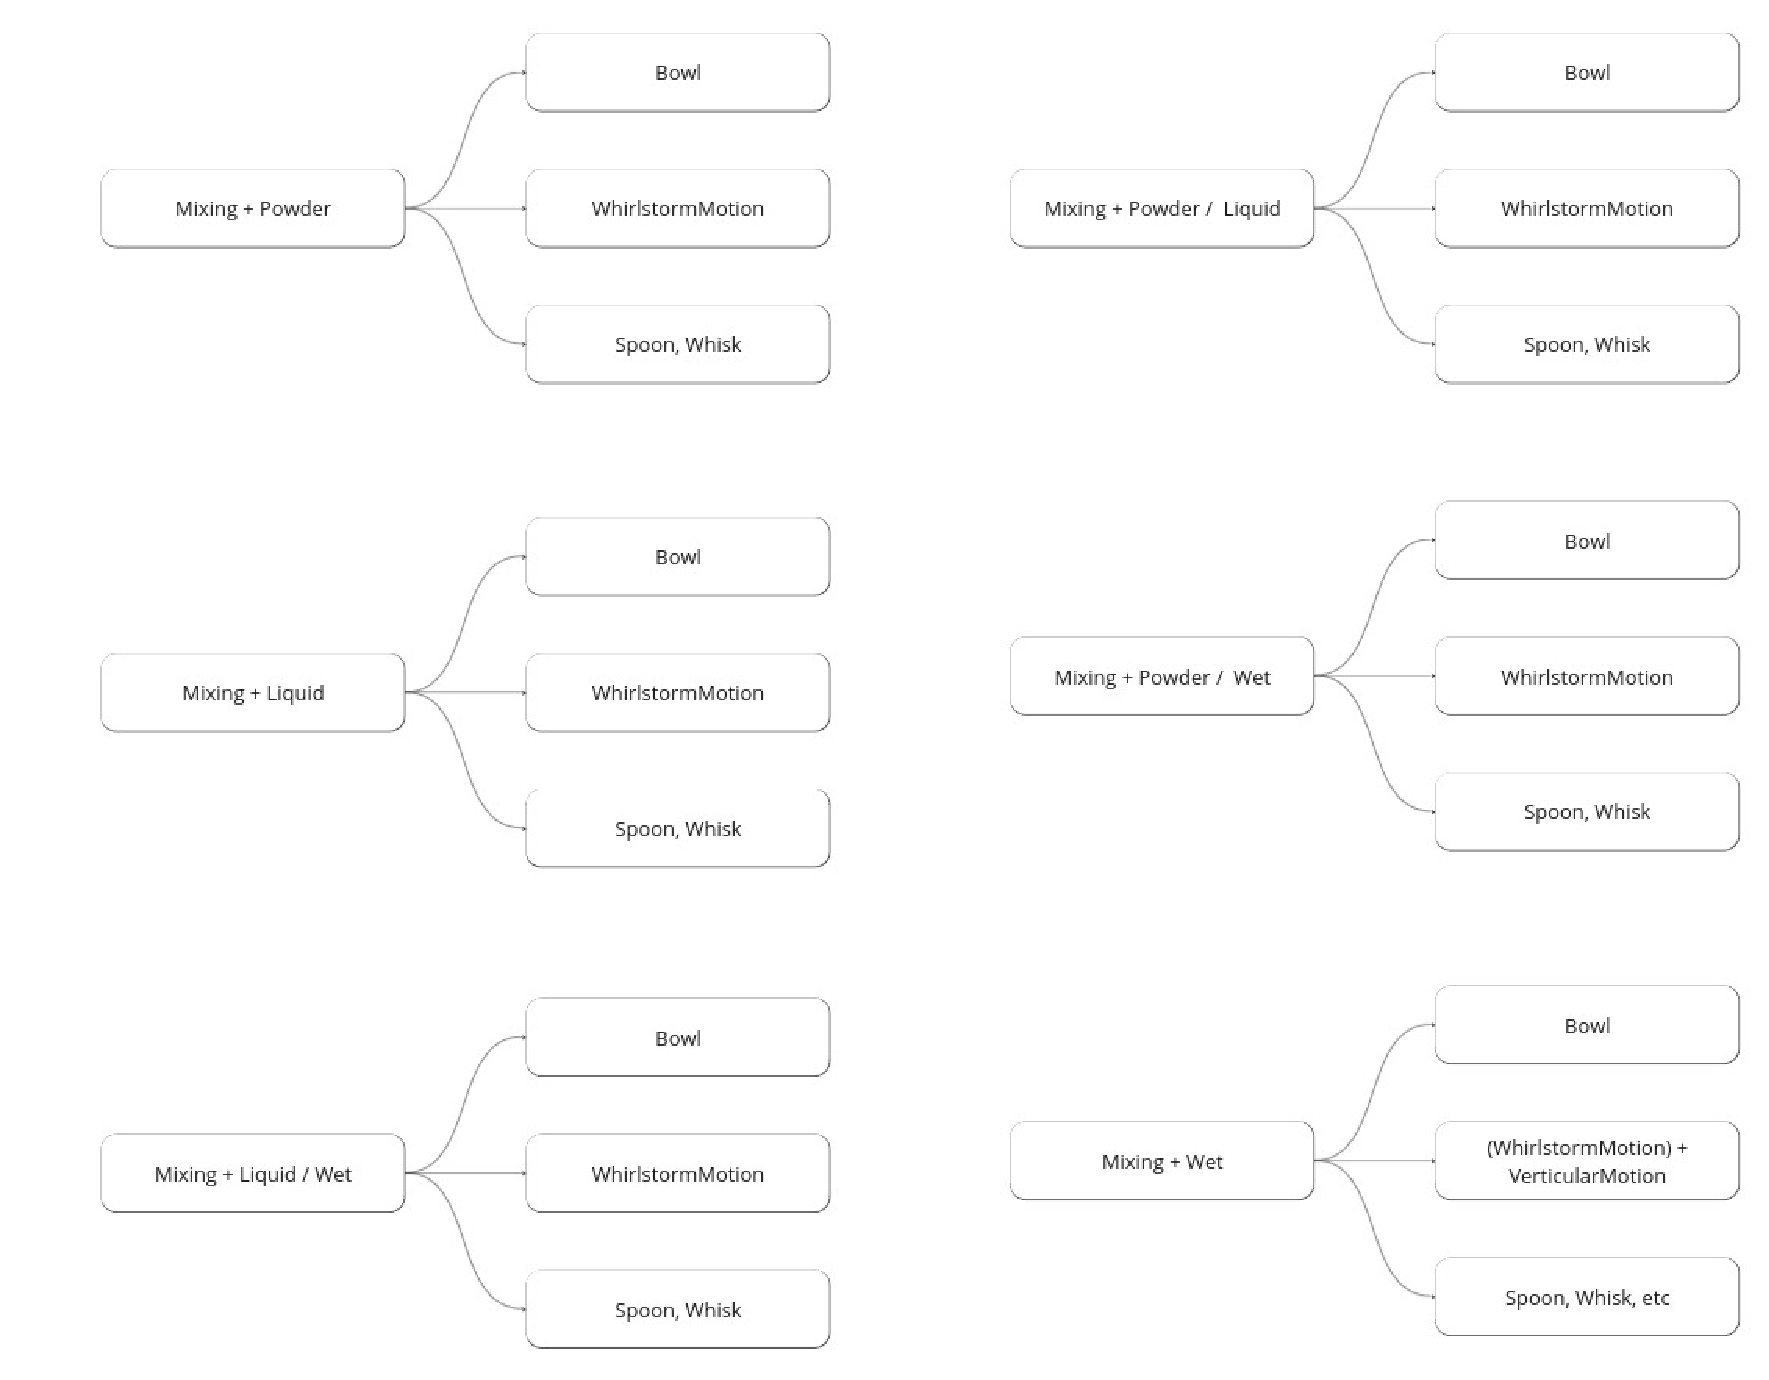
\includegraphics[scale=0.5]{Graphics/MixingDT.pdf}
\end{figure}

\subsection*{Stiring}
\begin{figure}[H]
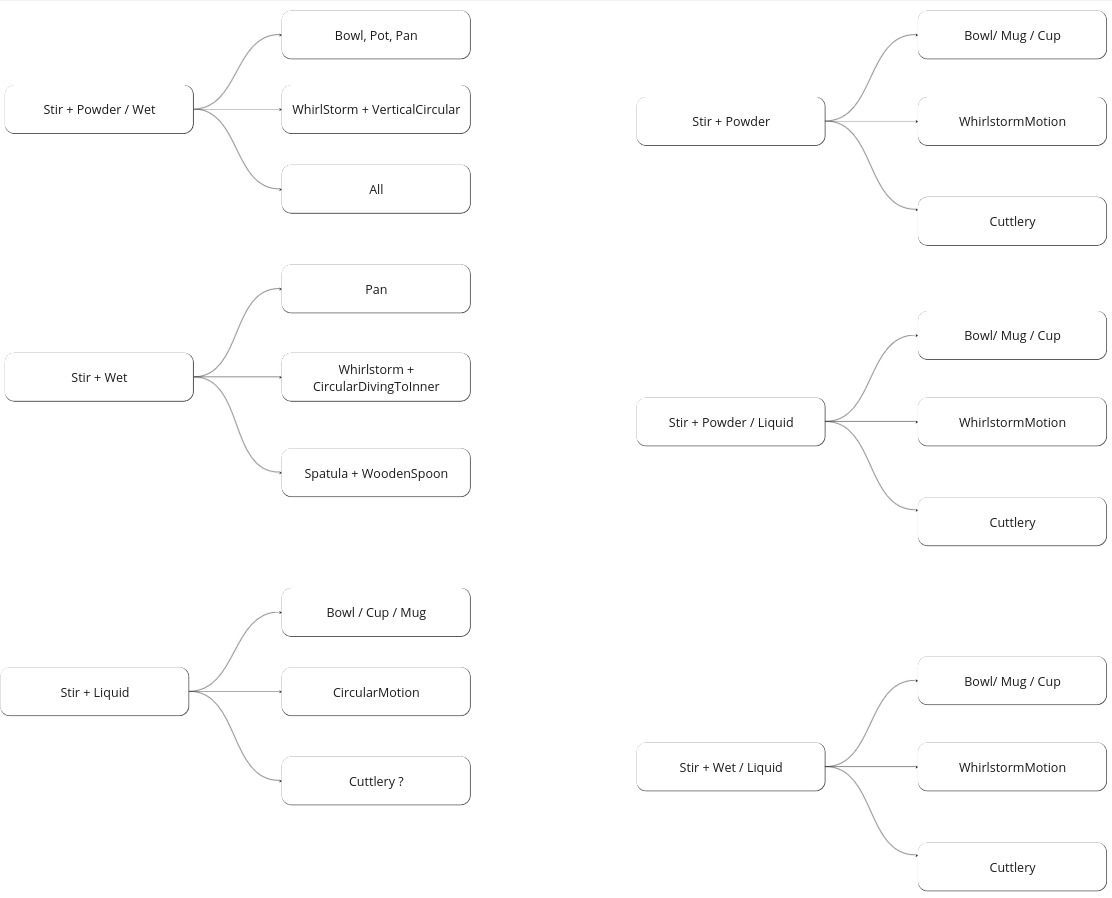
\includegraphics[scale=0.4]{Graphics/StirringDT.jpg}
\end{figure}


\subsection*{Beating}
\begin{figure}[H]
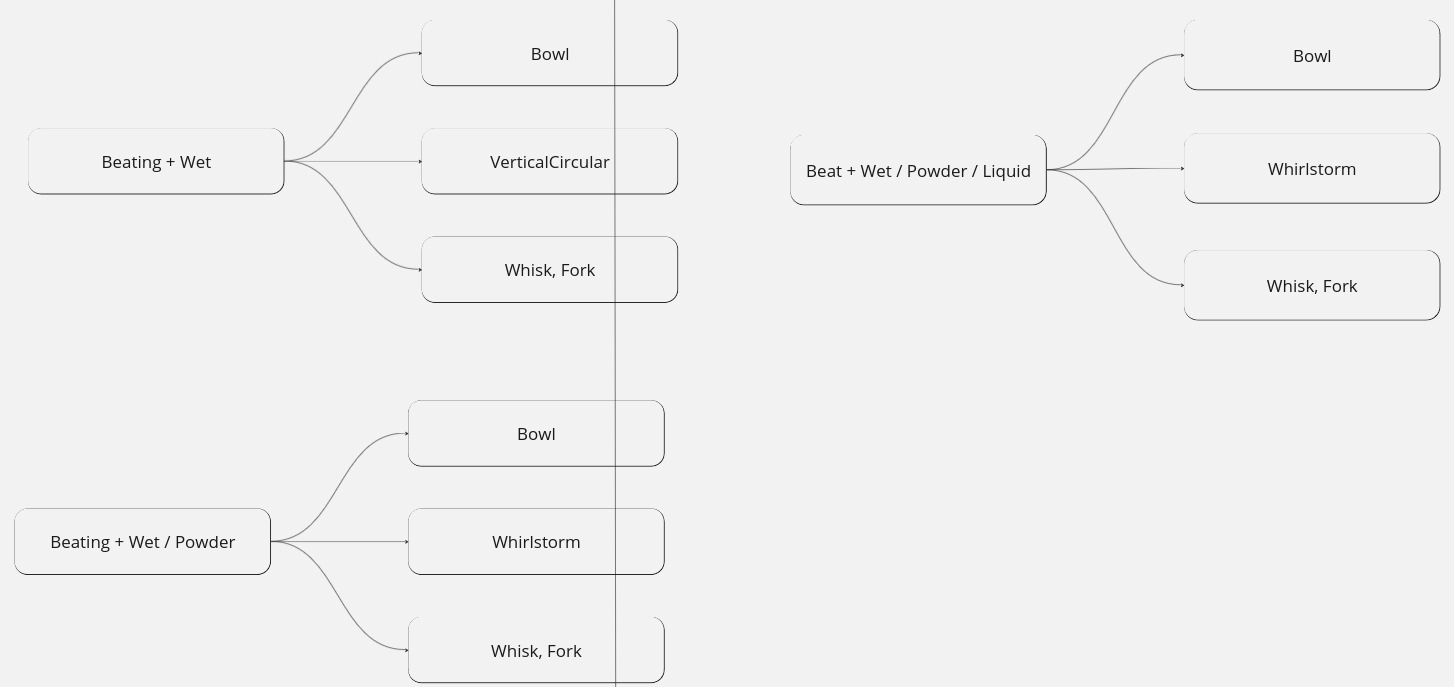
\includegraphics[scale=0.3]{Graphics/BeatingDT.jpg}
\end{figure}

\subsection*{Whisking}
\begin{figure}[H]
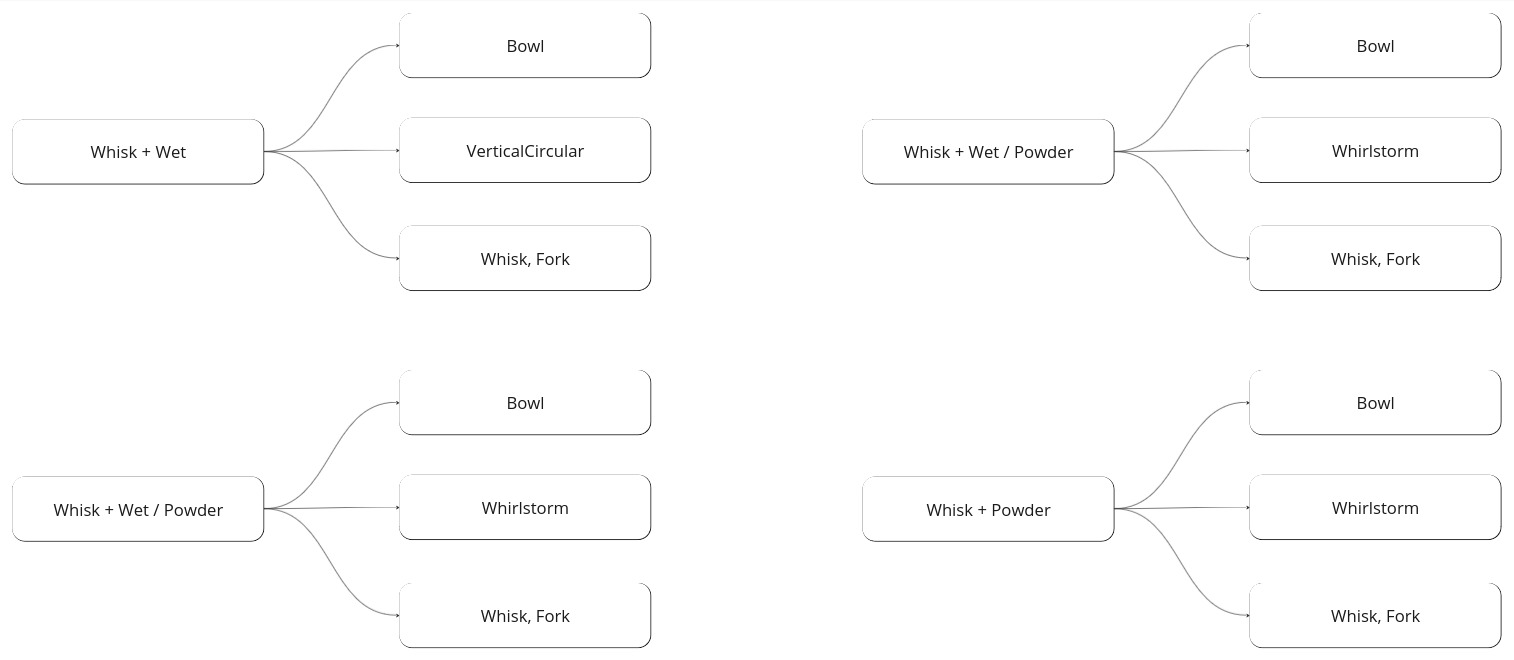
\includegraphics[scale=0.3]{Graphics/WhiskingDT.jpg}
\end{figure}